%
% File acl2021.tex
%
%% Based on the style files for EMNLP 2020, which were
%% Based on the style files for ACL 2020, which were
%% Based on the style files for ACL 2018, NAACL 2018/19, which were
%% Based on the style files for ACL-2015, with some improvements
%%  taken from the NAACL-2016 style
%% Based on the style files for ACL-2014, which were, in turn,
%% based on ACL-2013, ACL-2012, ACL-2011, ACL-2010, ACL-IJCNLP-2009,
%% EACL-2009, IJCNLP-2008...
%% Based on the style files for EACL 2006 by 
%%e.agirre@ehu.es or Sergi.Balari@uab.es
%% and that of ACL 08 by Joakim Nivre and Noah Smith

\documentclass[11pt,a4paper]{article}
\usepackage[hyperref]{acl2021}
\usepackage[utf8]{inputenc}
%\usepackage[T1]{fontenc}
%\usepackage[encoding]{fontenc}
\usepackage{times}
\usepackage{latexsym}
\renewcommand{\UrlFont}{\ttfamily\small}
\usepackage{amsmath,amsfonts,amssymb}
\usepackage[noabbrev,capitalize]{cleveref}
\usepackage{xargs}
\usepackage{graphicx}
%\usepackage[colorinlistoftodos,prependcaption,textsize=tiny]{todonotes}
%\newcommandx{\jp}[2][1=]{\todo[linecolor=purple,backgroundcolor=purple!25,bordercolor=purple,#1]{#2}}

% This is not strictly necessary, and may be commented out,
% but it will improve the layout of the manuscript,
% and will typically save some space.
\usepackage{microtype}
\newcommand\jp[1]{\textbf{JP: #1}}

\usepackage{pgfplots}
\usepackage{pgfplotstable}
    \pgfplotsset{
        compat=1.9,
        compat/bar nodes=1.8,
    }
    \pgfplotstableread{
        lang natural hallucinated
        tur	100310 0
        olo	100062 0
        vep	100053 0
        sah	100046 0
        por	100041 0
        pol	100039 0
        ara	100027 0
        tyv	100015 0
        kmr	100003 0
        rus	100002 0
        spa	100001 0
        aym	100000 0
        deu	100000 0
        ces	94169 0
        krl	78673 0
        bul	39011 0
        nld	38827 0
        amh	32254 0
        heb	23204 0
        afb	22165 0
        arz	17683 0
        cni	13948 0
        ckb	11577 0
        ind	11072 0
        evn	5216 10000
        see	3801 10000
        ame	2524 10000
        itl	1246 10000
        syc	1217 10000
        bra	1082 10000
        ail	918 10000
        mag	854 10000
        vro	804 10000
        kod	323 10000
        sjo	290 10000
        gup	214 10000
        ckt	132 10000
        lud	128 10000
    }\testdata

\aclfinalcopy % Uncomment this line for the final submission
%\def\aclpaperid{***} %  Enter the acl Paper ID here

%\setlength\titlebox{5cm}
% You can expand the titlebox if you need extra space
% to show all the authors. Please do not make the titlebox
% smaller than 5cm (the original size); we will check this
% in the camera-ready version and ask you to change it back.

\newcommand\BibTeX{B\textsc{ib}\TeX}

\title{Training Strategies for Neural Multilingual Morphological Inflection}

\author{Adam Ek and Jean-Philippe Bernardy \\
	Centre for Linguistic Theory and Studies in Probability \\
	Department of Philosophy, Linguistics and Theory of Science \\
	University of Gothenburg \\
	\texttt{\{adam.ek,jean-philippe.bernardy\}@gu.se} \\}

\date{}

\begin{document}
\maketitle
\begin{abstract}
This paper presents the submission of team GUCLASP to SIGMORPHON
2021 Shared Task on Generalization in Morphological Inflection
Generation. 

We develop a single multilingual model for all languages and explore
several training strategies.

....
\end{abstract}

\section{Introduction}

%Changes in strings typically nakes itself known through two processes,
%morphological inflection and derivation. In morphological derivation a
%words part of speech is changed, while in inflection the grammatical
%functions of the word change.

Morphological inflection is the task of transforming a \emph{lemma} to
its \emph{inflected form} given a set of \emph{grammatical features}
(such as \texttt{tense} or \texttt{person}).  Different languages have
different strategies, or morphological processes such as affixation,
circumfixation, or reduplication among others
\cite{haspelmath2013understanding}, to transform a lemma into an
inflected form that expresses some grammatical features.  One way to
characterise how languages express grammatical features is a spectrum
ranging from agglutinative to isolating. In agglutinative languages
grammatical features are encoded as bound morphemes attached to the
lemma, while in isolating languages each grammatical feature is
represented as a lemma. Thus, languages in different parts of this
spectrum will have different strategies for expressing information
given by grammatical features.



%The worlds languages
%exhibit a large variety of morphological inflection strategies,
%including affixing, circumfixing and reduplication among others
%\cite{haspelmath2013understanding}, that a system needs to address.
%\jp{citation(s) needed}.

%Additionally, languages fall into a spectrum ranging from agglutinative
%to isolating. In agglutinative languages grammatical features are
%encoded as bound morphemes attached to the lemma, while in isolating
%languages each grammatical feature is represented as a lemma. Thus,
%languages in different parts of this spectrum will have different
%strategies of incorporating information given by grammatical features.

In recent years, statistical and neural models have been performing
very well on this task \cite{DBLP:conf/eacl/SmitVGK14,
kann2016med}. We follow this tradition and implement a neural
multilingual model for morphological inflection. In a multilingual
system, a single model is developed to process multiple languages,
such that we can give it either a word in for example Swedish or
Evenk, which will be inflected.



%Several systems for inflecting words have been implemented both using
%statistical \cite{DBLP:conf/eacl/SmitVGK14, kann2016med} and
%rule-based methods \cite{DBLP:phd/basesearch/Hulden09}. In rule-based
%methods rules for transformatoins of strings are identified and
%applied accordingly. In this paper we focus on morphological
%inflection with neural networks, specifically, a multilingual
%system. In a multilingual system, a single model is developed to
%process multiple languages, such that we can give it either a word in,
%for example, Swedish or Evenk that will be inflected.  

This is a challenging problem for several reasons. For many languages
resources are scarce, and a multilingual system must try the balance
the training signals from both high-resource and low-resource
languages such that the model learns something about both.
Additionally, different languages employ different morphological
processes to inflect words. In addition to languages employing a
variety of different morphological processes, different languages use
different scripts (for example Arabic, Latin, or Cyrillic), which can
make it hard to transfer knowledge about one language to another.  To
account for these factors a model must learn to recognize the
different morphological processes, their associated grammatical
features, the script used, and map them into individual languages.

In this paper, we investigate how far these issues can be tackled
using different training strategies, as opposed to focusing on model
design. Of course, in the end an optimal system will be a
combination of a good model design and good training strategies.
% \adam: add something here

%However, an advantage of finding good training strategies is that they
%do not (generally) require additional parameters in the model. This
%allows a model to obtain better representations with fewer parameters,
%thus increasing the quality of representations without needing
%too many additional encoding parameters.


%In this paper we explore different training schemas for neural
%networks, in a multilingual model for morphological inflection in 37
%different languages.

%We are particularly interested in how far we can get using a simple
%LSTM sequence-to-sequence model with attention, augmented with
%training procedures informed by human heuristics.

We employ an LSTM encoder-decoder architecture with attention, based on
the architecture in \newcite{DBLP:conf/emnlp/AnastasopoulosN19}, as our
base model and consider the following training strategies:

\begin{itemize}
\item Curriculum learning: We augment the order in which the examples are presented to the model based on the loss.
\item Multi-task learning: We predict the formal operations required to transform a lemma into its inflected form.
\item Language-wise label smoothing: We smooth the loss function to not penalize the model as much when it predicts a character from the correct language.
\item Scheduled sampling: We use a probability distribution to determine whether to use the previous output or the gold as input when decoding.
\end{itemize}

%\section{Task} moved to beginning of intro
%As mentioned previously the task of morphological inflection is to
%predict the \emph{inflectional form} of a lemma (the ``base'' form of
%a word) given a set of grammatical features (such as \texttt{tense} or
%\texttt{person}).
%
%- tag
%- lemma
%- prediction (inflected form)

%[perhaps: Describe edition tasks here as well (as auxiliary tasks)]

\section{Data}

The data released cover $38$ languages of varying typology, genealogy,
grammatical features, scripts, and morphological processes. The data
for the different languages vary greatly in size, from $138$ examples
(Ludic) to $100310$ (Turkish).  For the low-resourced
languages\footnote{We consider languages with less than 10 000
training examples as low-resource in this paper.} we produce
\textbf{hallucinated data} to train on. We follow
\cite{DBLP:conf/emnlp/AnastasopoulosN19}, and produce a new inflected
form by replacing the parts of an existing inflected form that
overlap with the lemma.

With respect to the work of \citet{DBLP:conf/emnlp/AnastasopoulosN19},
we make the following changes. We identify all subsequences of length
$3$ or more that overlap in the lemma and inflection. We then randomly
sample one of them, denoted $R$, as the sequence to be replaced.  For
each language, we compile a set $\mathcal{C_L}$ containing all
(1,2,3,4)-grams in the language. We construct a string $G$ to replace
$R$ with by uniformly sampling \textit{n}-grams from $\mathcal{C}$ and
concatenating them $G = g_0, ..., g_m$ until we have a sequence whose
length satisfy: $|R|-2 \leq |(g_0, ..., g_m)| \leq |R|+2$.

%To generate a new
%subsequence we randomly sample a set $G$ of 

%we randomly sample $n$ (1,2,3,4)-grams in the language
%such that $|r|-2 \leq |(g_0, ..., g_n)| \leq |r|+2$ and replace $r$
%with the concatenation of $(g_0, ..., g_n)$. % fix notation...

Additionally, we don't consider subsequences which include a
phonological symbol \footnote{Thus in \cref{fig:hall} a subsequence of
length 2 is selected as the sequence to be replaced, since the larger subsequences
would include the phonological symbol :}.  A schematic of the hallucination
process is shown in \cref{fig:hall}.


\begin{figure}[h]
\centering
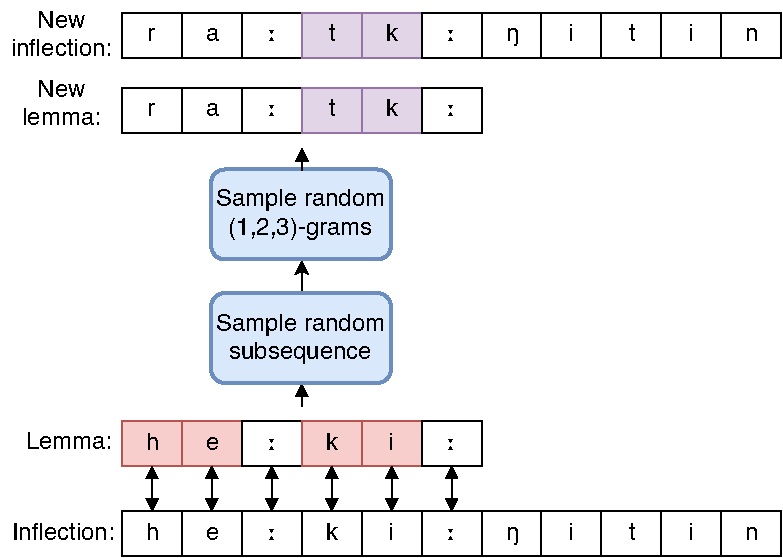
\includegraphics[scale=0.5]{hall.pdf}
\caption{\label{fig:hall} A example of the data hallucination process. The sequence $R=\text{ki}$ is replace by $G=\text{tk}$.}
\end{figure}


For each language with fewer than 10 000 examples, we sample 10 000
new examples. A visualization of the final number of examples in each
language is shown in \cref{fig:data}.

\begin{figure}[ht]
\begin{tikzpicture}
    \begin{axis}[
        ybar stacked,
        ymin=0,
        ymax=105000,
        scaled y ticks={false},
        xtick=data,
        legend style={
            cells={anchor=west},
            legend pos=north east,
        },
        width=\columnwidth*1.15,
        height=100pt,
        /pgf/bar width=4pt,
        reverse legend=true,
        xticklabels from table={\testdata}{lang},
        xticklabel style={text width=1cm,align=center,font=\tiny,rotate=90},
        yticklabel style={text width=1cm,align=center,font=\tiny,rotate=90}
    ]
        \addplot [fill=green!50]
            table [y=natural, meta=lang, x expr=\coordindex]
                {\testdata};
                    \addlegendentry{natural}
        \addplot [fill=blue!50]
            table [y=hallucinated, meta=lang, x expr=\coordindex]
                {\testdata};
                    \addlegendentry{hallucinated}
    \end{axis}
\end{tikzpicture}
\caption{\label{fig:data} Number of natural and hallucinated examples in each language.}
\end{figure}


%We improve upon [REF] in the following way.
%Noting that certain languages in the data use phonological symbols
%and separators, we hallucinate in such a way that we don't break apart
%morphemes.


\section{Method}

In this section, the multilingual model and training strategies used
are presented. We employ a single model with shared parameters
across all languages. 

\subsection{Model}

We can account for different languages in our single model in several
ways, in this paper we use a language embedding as the first position
in the representation of the lemma and inflection.

% We use a language embedding as the first position in our input, thus
% the input is $[lang_{id}, emb_{c_0},..., emb_{c_n}]$.

We employ an encoder-decoder architecture with attention. The first
layer in the model is comprised of an LSTM, which produces a
contextual representation for each character in the lemma.

We encode the tags using a self-attention module (equivalent to a
1-head transformer layer).  This layer does not use any positional
data: indeed the order of the tags does not matter (REF).

We use an LSTM decoder with two attention modules. One attending to
the lemma and one to the tags. For the lemma attention, we use a
content-based attention module \cite{graves2014neural,
karunaratne2021robust} which uses cosine similarity.  However, we
found that using content-based attention only causes attention to be
too focused on a single character, and mostly ignores contextual cues
relevant for the generation.

To remedy this, we combine the content-based attention with additive
%attention as follows, where superscript $cos$ indicate cosine
%attention, $add$ additive attention, $h_t$ the hidden state from the
%encoder, $h_d$ the previous time-step from the decoder and $k$ the
%key:
%\jp{
%  1. Double-check the code.
%  2. Use another naming than additive (I think it's multiplicative)}
attention as follows, where superscript $cb$ indicate content-based attention,
$add$ additive attention and $k$ the key:

\begin{align*}
	a^{add} & = \mathsf{softmax}(w^\top\mathsf{tanh}(\mathsf{W}_ak + \mathsf{W}_bh))\\
	att^{add} & = \sum_{t=1}^{T}a_t^{add}h_t^{add}\\
	a^{cb} & = \mathsf{softabs}(cos(k,h))\\
	att^{cb} & = \sum_{t=1}^{T}a_t^{cb}h_t^{cb}\\
	att & = \mathsf{W}[att^{cb}; att^{add}]
\end{align*}
%(in the above $h_t$ refers to the encoder's contextual representation for each character.)
We employ additive attention for the tags. In each decode-step we pass the
concatenation of the character embedding obtained from the previous
step, the lemma attention, and the tag attention to the decoder.

% \[\text{input}_t = [e_{t-1}; att_{char}; att_{tag}]\]

\subsection{Multi-task learning}

Instead of predicting the inflected form, one can also predict the
Levenshtein operations needed to transform the lemma into the
inflected form; as inspired by \cite{DBLP:conf/conll/MakarovRC17}.

A benefit of considering operations instead of characters needed to
transform a lemma to its inflected form is that the script used is a
much lesser factor here. We find that making \emph{both} predictions,
as a multi-task setup, improves the performance of the system.

The multi-task setup operates on the character level, thus for each
contextual representation of a character we want to predict an
operation among \textit{deletion} (\texttt{del}),
\textit{addition/insetion} (\texttt{add}), \textit{substitution}
(\texttt{sub}) and \textit{copy} (\texttt{cp}). Because \texttt{add}
and \texttt{del} change the length, we predict two sets of operations,
the \textbf{lemma-reductions} and the \textbf{lemma-additions}. To
illustrate, the levenshtein operations for the word pair
(\emph{valatas}, \emph{ei valate}) in Veps (uralic language related to
Finnish) is shown in \cref{fig:ops}.

%We break down the task of applying levenshtein-distance operations
%into two sub-tasks: \textbf{lemma-reductions}, where we predict the copy and
%deletion operations and \textbf{lemma-additions}, where we predict the copy and
%addition operations. 

\begin{figure}[ht]
\centering
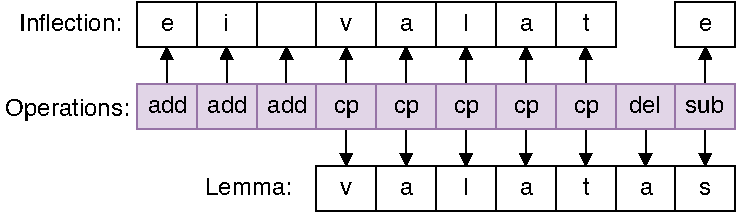
\includegraphics[scale=0.5]{ops.pdf}
\caption{\label{fig:ops} Levenshtein operations mapped to characters in the lemma and
inflection.}
\end{figure}

In our setup, the task of lemma-reductions is performed by predicting
the \texttt{cp}, \texttt{del}, and \texttt{sub} operations based on
the encoded hidden states in the lemma.  The task of lemma-additions
then is performed by predicting the \texttt{cp}, \texttt{add}, and
\texttt{sub} operations on the characters generated by the decoder.
We use a single 2-layer perceptron with ReLU activation to predict
both lemma-reduction and lemma-additions. \footnote{In the future,
we'd like to experiment with including the representations of tags in
the input to the operation classifier.}


%\jp{I don't see how this solves the length problem?}
%To predict the operations, we pass the lemma representations from the
%encoder and the generated inflection representations to a single operation
%classification layer.

%For each sub-task we predict the operation based on the hidden states
%generated by our neural network. In the case of lemma-reductions we
%predict the operation on the hidden-states of the encoded lemma. For
%lemma-additions, we predict the operations on the generated characters
%from the decoder.

\subsection{Curriculum Learning}

%We employ a simple curriculum learning strategy where we 
%sort the data after each epoch based on the loss of each example. For
%all examples in the batch we sort them according to the loss obtained
%in the previous epoch, in ascending order such that the easy (low
%loss) occurs before the difficult examples (high loss).

We employ a competence-based curriculum learning strategy based on the
work of \cite{DBLP:conf/acl/LiuLWC20} and
\cite{platanios2019competence}. A competence curriculum learning
strategy construct a curriculum based on the \textit{competence} of a
model, and present examples which the model is deemed to be able to
handle. Thus, the model will gradually be presented with new more
difficult examples. The goal of this strategy is for the model to
transfer or apply the knowledge it acquired from the easy examples to
the hard examples.
 
To estimate an initial difficulty for an example we consider the
unigram probability of the lemma and inflection. That is for a word
(either the lemma or inflection) $c_0, ..., c_k$, the unigram log
probability is given by:

\begin{equation}
    P_U(w) = \sum_{m=1}^{M} logp(c_i)
\end{equation}

To get a score for a lemma and inflection pair (henceforth $(x,y)$),
we calculate it as the sum of the log probabilities of $x$ and $y$:

\begin{equation}
    score(x,y) = P_U(x) + P_U(y)
\end{equation}

We then sort the examples and use a cumulative density function to map
the unigram probabilities to a score in the range $(0, 1]$, we denote
the training set of pairs and their scores
$((x,y), s)_0, \ldots, ((x,y), s)_m$, where $m$ indicate the number of
examples in the dataset, as $\mathcal{D}$.

%We create a curriculum learning schedule by considering the
%\textit{model competence}-based approach
%\cite{platanios2019competence}.
% 
%A model competence approach to
%curriculum learning defines a ``initial'' competence of a model which
%determines which examples in the training set the model is competent
%enough to train on at time-step $t$.
%
To select appropriate training examples from $\mathcal{D}$ we must
estimate the competence $c$ of our model. The competence of the model
is estimated by a function of the number of training steps $t$ taken:

%We take the competence of the model to be
%a fuction of the number of training steps $t$ taken

%The competence $c$ of the model is gradually increased as a function
%of the training steps $t$ taken [REF], thus:

\begin{equation}
    c(t) = \mathsf{min}(1, \sqrt{t\frac{1-c(1)^2}{c(1)^2}+c(1)^2})
\end{equation}

During training, we employ a probabilistic approach to constructing
batches from our corpus, we uniformly draw samples $((x, y), s)$ from
the training set $\mathcal{D}$ such that the score $s$ is lower than
the model competence $c(t)$. This ensures that for each training
step, we only consider examples that the model can handle according
to our curriculum schedule.

However, just because an example has low unigram probability doesn't
ensure that the example is easy, as the example may contain frequent
characters but also include rare morphological processes (or rare
combinations of Levenshtein operations), to account for this we
recompute the example scores for each training step. We sort the
examples in each training step according to the \textbf{decoding
loss}, then assign a new score to the batch examples in the range
$(0, 1]$.

We also have to take into account that as the model competence grows,
``easy'' (low loss or high unigram probability) examples will be
included more often in the batches. To ensure that the model learns
more from examples whose difficulty is close to its competence we
compute a weight $w$ for each example in the batch. We then scale the
loss by dividing the score $s$ by the model competence at the current
time-step:

\begin{equation}
\mathsf{weighted\ loss}(x, y) = \mathsf{loss}(x, y) \times \frac{score(x, y)}{c(t)}
\end{equation}

%Remember, we recompute the difficult of each example at every training
%step, assigning it a new score in the range $(0, 1]$.



%For the first epoch, when we dont have any loss refer to for sorting,
%we sort the dataset according to the ratio of copy operations to other
%operations. We found that this strategy performed better than any of
%the other strategies which we tested: fewest addition-operations,
%least-grammatical-features, and random.  This strategy causes a small,
%but consistent improvement in the loss of the first epoch, which
%persists throughout the learning process.\jp{Curriculum learning in
%general or the specific thing for the 1st epoch? Adam: Currently
%reconsidering this approach in favor of something cooler}

\subsection{Scheduled Sampling}

Commonly, when training an encoder-decoder RNN model, the input at
time-step $t$, is not the output from the decoder at $t-1$, but rather
the gold data.  It has been shown that models trained with this
strategy may suffer at inference time. Indeed, they have never been
exposed to a partially incorrect input in the training phase.  To
address this issue we use scheduled sampling
\cite{DBLP:conf/nips/BengioVJS15}.

We implement a simple schedule for calculating the probability of
using the gold characters or the model's prediction by using a global
sample probability variable which is updated at each epoch. We start
with a probability \(\rho\) of 100\% to take the gold. At each epoch,
we decrease \(\rho\) by 4\%. For each character, we take a sample from
the Bernoulli distribution of parameter \(\rho\) to determine the
decision to make.

\subsection{Training}

We use cross-entropy loss for the character generation loss and 
%We use KL-divergence loss for the characters
%\jp{But the entropy of the
%  label distribution is constant? So this is a red flag. If it's a
%  workaround for a bug in pytorch, this should come down to a
%  footnote.} 
%and cross-entropy loss 
for the operation predictions tasks. Our final loss function consists
of the character generation loss, the lemma-reduction and the
lemma-addition losses summed.

\paragraph{Language-wise Label smoothing} We use language-wise label
smoothing to calculate the loss. This means that we remove $\alpha$
from the probability of the correct character and distribute the same
$\alpha$ uniformly across the probabilities of the characters
belonging to the language of the word. A difficulty is that each
language potentially uses a different set of characters. We calculate
this set using the training set only--- so it is important to make
$\alpha$ not too large, so that there is not a too big difference
between characters seen in the training set and those not seen.
Indeed, if there were, the model might completely exclude unseen
characters from its prediction at test-time. (We found that
\(\alpha=2.5\%\) is a good value.)

\paragraph{Learning rate decay with a Curriculum} Recall that the
training examples will be sorted by the difficulty in the previous
epoch.  We note that employing a decaying learning rate has the effect
that a model updates its parameters \emph{more} on the easy examples
and less on the difficult examples. The idea is that the morphological
processes involved in more difficult words can be discovered from the
operations involved in the easier examples.

The hyperparameters used for training are presented in \cref{tab:hp} below.
\begin{table}[h]	
\centering
\begin{tabular}{lc}
\textsc{Hyperparameter} & \textsc{Value} \\
  \hline
  Batch Size & 256 \\
  Embedding dim & 128 \\
  Hidden dim & 256 \\
  Epochs & 30 \\
  Initial LR & 0.001 \\
  Min LR & 0.0000001 \\
  Smoothing-$\alpha$ & 2.5\% \\
\end{tabular} 
\caption{Hyperparameters.}
\label{tab:hp}
\end{table}

\section{Results}

The results from our system are presented in \cref{tab:accuracy}. For
each language in the training set we show the exact match accuracy and
the levenshtein edit distance between the lemma and the inflected
form.


\begin{table}[ht!]	
\centering
\begin{tabular}{lc}
\textsc{Lang} & \textsc{EM} \\
  \hline
  tur	& 100310  \\
  olo	& 100062  \\
  vep	& 100053  \\
  sah	& 100046  \\
  por	& 100041  \\
  pol	& 100039  \\
  ara	& 100027  \\
  tyv	& 100015  \\
  kmr	& 100003  \\
  rus	& 100002  \\
  spa	& 100001  \\
  aym	& 100000  \\
  deu	& 100000  \\
  ces	& 94169  \\
  krl	& 78673  \\
  bul	& 39011  \\
  nld	& 38827  \\
  amh	& 32254  \\
  heb	& 23204  \\
  afb	& 22165  \\
  arz	& 17683  \\
  cni	& 13948  \\
  ckb	& 11577  \\
  ind	& 11072  \\
  evn	& 5216  \\
  see	& 3801  \\
  ame	& 2524  \\
  itl	& 1246  \\
  syc	& 1217  \\
  bra	& 1082  \\
  ail	& 918  \\
  mag	& 854  \\
  vro	& 804  \\
  kod	& 323  \\
  sjo	& 290  \\
  gup	& 214  \\
  ckt	& 132  \\
  lud	& 128  \\
\end{tabular} 
\caption{Acc}
\label{tab:accuracy}
\end{table}



\subsection{Ablation Study}

We perform a leave-one-out ablation study to estimate the effect of
our proposed training strategies.

%\jp{Not sure if ablation is the right word here.}

\begin{table}[ht!]	
\centering
\begin{tabular}{lr}
\textsc{Module} & \textsc{avg. EM}\\
  \hline
  All  & $76.4$ \\
  w/o Curriculum learning & $75.5$\\
  w/o Label smoothing & $72.7$\\
  w/o Multitask & $74.6$ \\
  w/o Scheduled sampling & $75.5$ \\  
\end{tabular} 
\caption{We evaluate the ablation experiment by calculating the exact
match accuracy for each language, then taking the mean over all
languages.}
\label{tab:abl}
\end{table}

The experiment shows that curriculum learning and scheduled sampling
both degrade the performance by $0.9$ percentage points. Removing the
prediction of operations, i.e. \texttt{del}, \texttt{add} and so on
degrade the performance more with a change of $-1.8$ percentage
points. Lastly, removing the language-wise label smoothing resulted in
a change of $-3.7$ percentage points. 

%Our implementation of curriculum learning is simplistic and does not
%include refinements such as model competence threshold and advanced
%scoring which may explain the lesser impact. 

The scheduled learning module also doesn't add that much to our
model. We hypothesise this is because the low-resource languages
benefit from using the gold as input when predicting the next
character, while high-resource languages do not need this as
much. The model has seen more examples from high-resource languages
and thus can model them better, which makes using the previous
hidden state more reliable as input when predicting the next token.

- analysis: language embeddings TSNE
- analysis: character embeddings TSNE

\section{Conclusions and future Work}

We presented 


\section*{Acknowledgments}

The research reported in this paper was supported by grant 2014-39
from the Swedish Research Council, which funds the Centre for
Linguistic Theory and Studies in Probability (CLASP) in the Department
of Philosophy, Linguistics, and Theory of Science at the University
of Gothenburg.

 
\bibliographystyle{acl_natbib}
\bibliography{acl2021}

%\appendix



\end{document}
